%
%
% Kapitel MC-Studien
%
%


\chapter{Studie der von WHIZARD generierten Monte-Carlo-Samples}

Die Studie der von WHIZARD generierten MOnte-Carlo-Daten soll zeigen, wie sich der Wirkungsquerschnitt des $t\overline{t}+\gamma$-Prozesses sowie das $E_T$-Spektrum der Photonen aus dem harten Prozess durch Variation des angenommenen $d_A^{\gamma}$-Wertes ver�ndert. Des weiteren soll untersucht werden, welche Variable sich am besten dazu eignet, zwischen verschiedenen $d_A^{\gamma}$-Szenarien zu unterscheiden. Durch Verwendung von Generatorteilchen werden Aufl�sungseffekte durch die Rekonstruktion sowie Akzeptanzeffekte durch die Selektion vernachl�ssigt.

\section{Wirkungsquerschnitt des \texorpdfstring{$t\overline{t}+\gamma$}{ttg}-Prozesses}

Es wird eine quadratische Abh�ngigkeit des Wirkungsquerschnittes vom Parameter $d_A^{\gamma}$ erwartet, da $d_A^{\gamma}$ linear in das Matrixelement eingeht und der Wirkungsquerschnitt proportional zum Quadrat des Matrixelementes ist. \\
Mit dem Leading-Order-Monte-Carlo-Generator WHIZARD in der Version 2.1.1 werden f�r Werte f�r das elektrische Dipolmoment von $0<d_A^{\gamma}<1$ in Schritten von 0,01 zun�chst die Matrixelemente f�r den harten Prozess generiert. Der Ansatz $2 \rightarrow 5$ wird implementiert mit zwei W-Bosonen, zwei b-Quarks und einem Photon im Endzustand. Die Matrixelement-Berechnung wird abgebrochen, wenn ein Fehler auf den Wirkungsquerschnitt von unter 1\% errechnet wird. Die so berechneten Wirkungsquerschnitte sind in Abb. \ref{fig:cs_wofit} links dargestellt. Man erkennt die erwartete quadratische Abh�ngigkeit. Fittet man eine quadratische Funktion an die Verteilung (Abb. \ref{fig:cs_wofit}), wird diese Abh�ngigkeit noch deutlicher.

\begin{figure}%
\centering
\begin{subfigure}[b]{0.4\textwidth}
  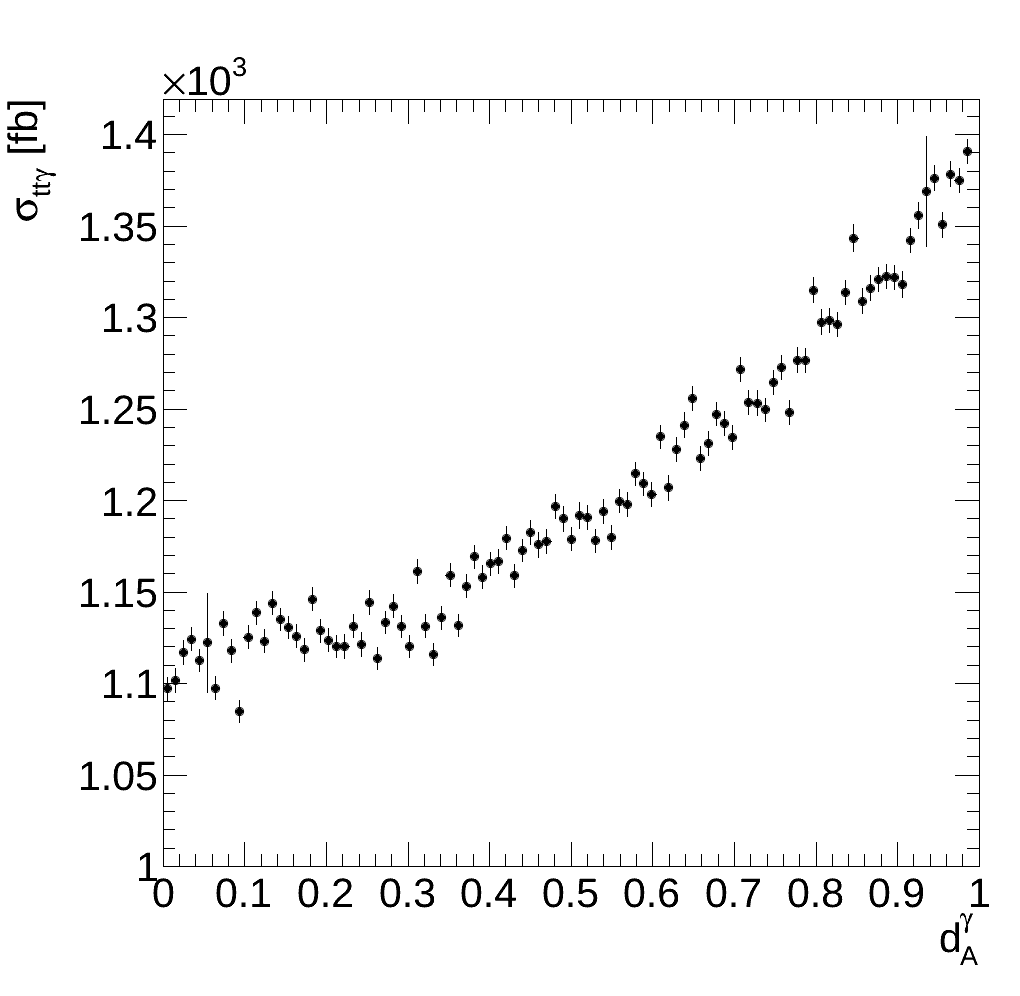
\includegraphics[width=\textwidth]{bilder/csplotwofit}%
\end{subfigure}
\hspace{0.1\textwidth}
\begin{subfigure}[b]{0.4\textwidth}
  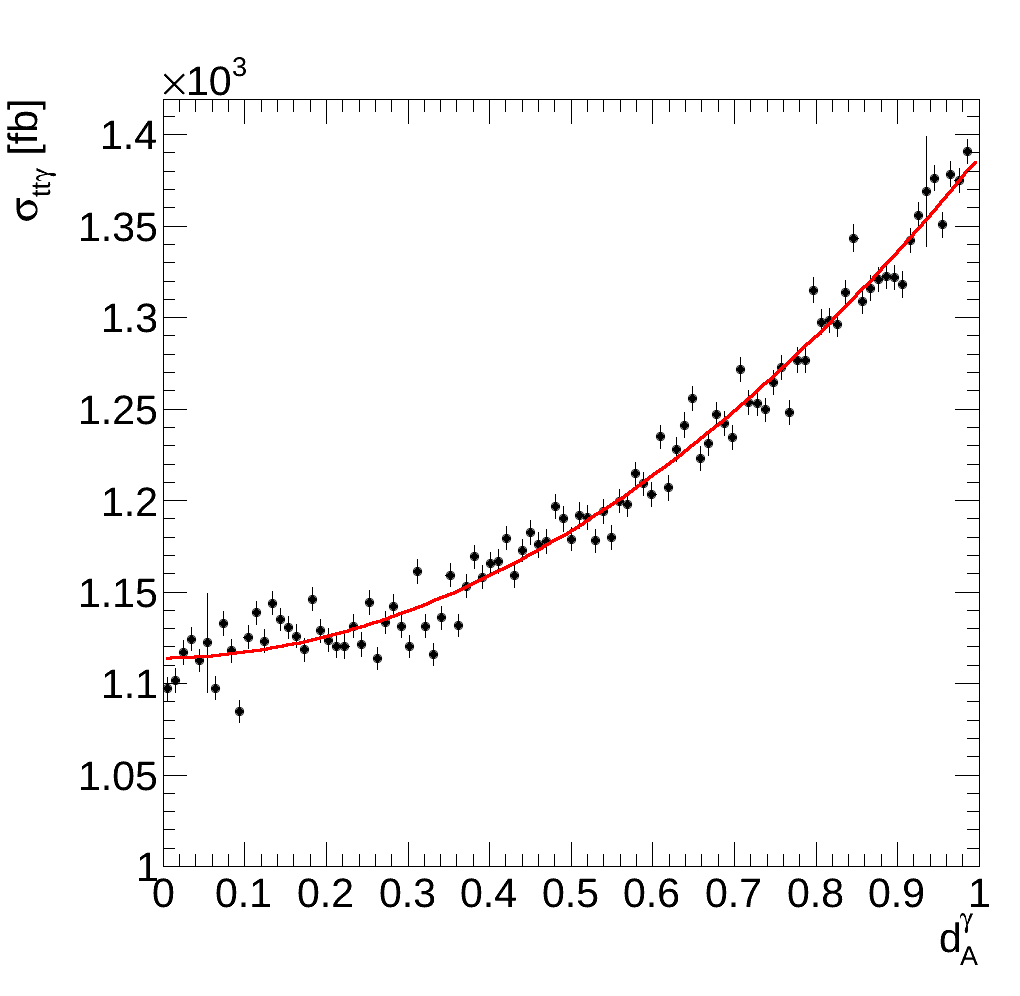
\includegraphics[width=\textwidth]{bilder/crosssectionplot}%
\end{subfigure}	
\caption{Wirkungsquerschnitt des $t\overline{t}+\gamma$-Prozesses f�r $0<d_A^{\gamma}<1$, rechts mit eingezeichneter Fit-Funktion}%
\label{fig:cs_wofit}%
\end{figure}

\section{\texorpdfstring{$E_T$}{ET}-Spektrum des Photons}

Aus dem berechneten Matrixelement werden nun f�r jeden $d_A^{\gamma}$-Wert 105.000 Ereignisse generiert und im Les-Houches-Event Format (LHEF) abgespeichert \cite{Alwall:LesHouches}. Es wird f�r ein h�heres elektrisches Dipolmoment ein h�rteres Photonspektrum erwartet. Um dies zu verifizieren, gibt es mehrere Ans�tze, die im Folgenden erl�utert werden sollen.

\subsection{2-Bin-Analyse}

Das $E_T$-Spektrum wird in zwei Bereiche aufgeteilt. Der erste Bereich reicht von 50\,GeV bis 100\,GeV, der zweite von 100\,GeV bis 200\,GeV, siehe dazu Abb. \ref{fig:2bin_skizze}. Nun wird das Verh�ltnis der Anzahl der Photonen in den beiden Bereichen gegen $d_A^{\gamma}$ aufgetragen, siehe Abb. \ref{fig:2bin_plot}.

\begin{figure}%
\centering
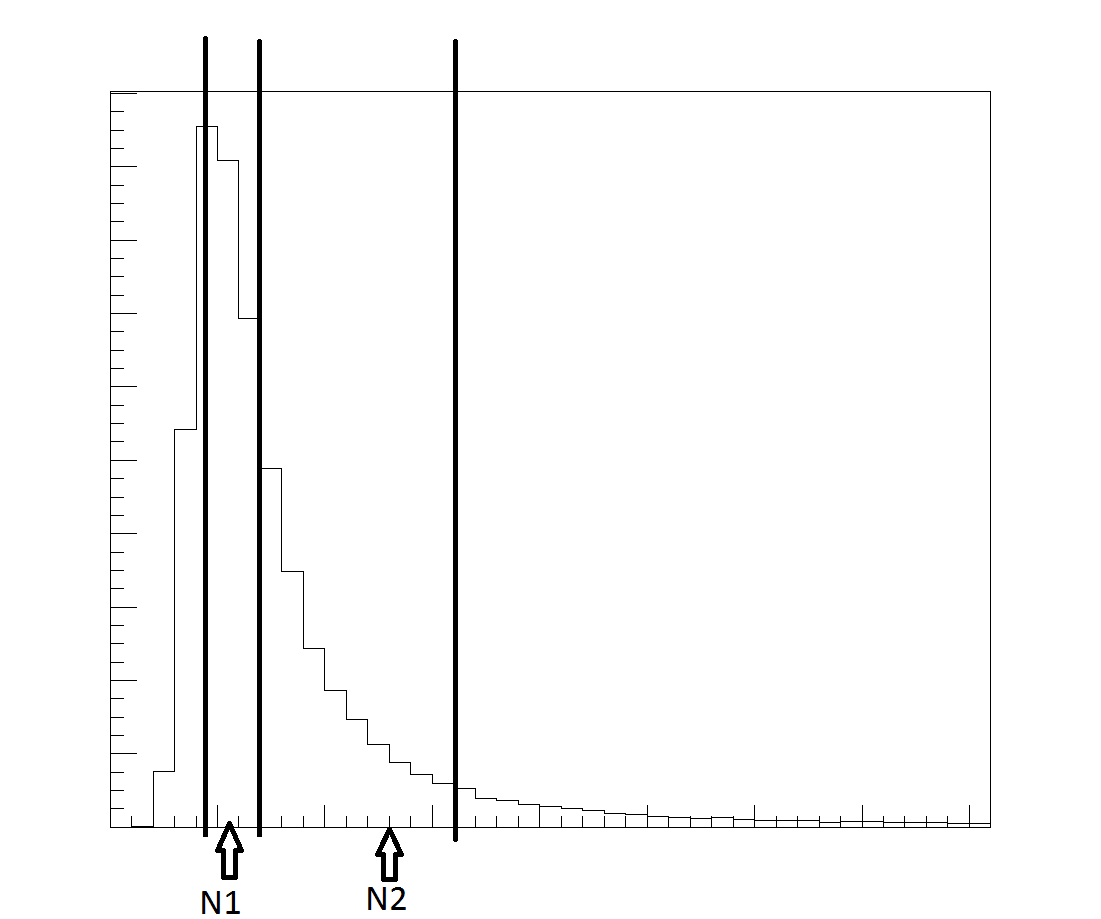
\includegraphics[width=0.5\columnwidth]{bilder/2binskizze}%
\caption{Schema der Unterteilung bei der 2-Bin-Analyse.}%
\label{fig:2bin_skizze}%
\end{figure}

\begin{figure}%
\centering
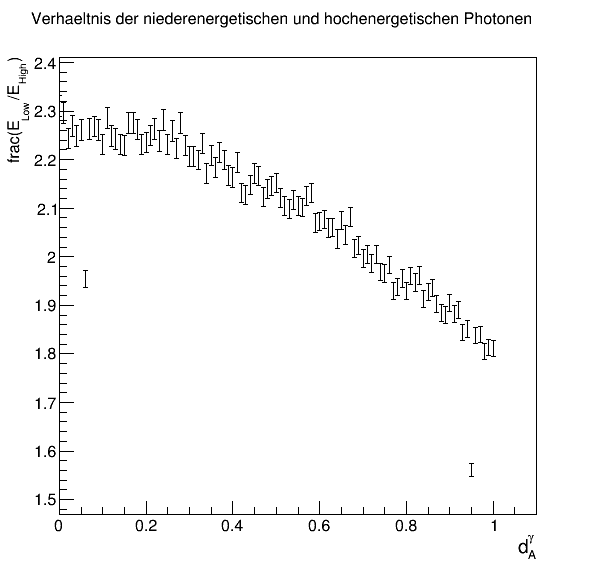
\includegraphics[width=0.5\columnwidth]{bilder/twobinplot}%
\caption{Verh�ltnis der Anzahl der Photonen in Bin 1 und Bin 2.}%
\label{fig:2bin_plot}%
\end{figure}

\subsection{\texorpdfstring{$E_T$}{ET}-Mean-Analyse}

In diesem Ansatz wird der Schwerpunkt der $E_T$-Verteilung betrachtet, siehe Abb. \ref{fig:mean_skizze}, dies ist der gewichtete Mittelwert dieser Verteilung. Mithilfe der Analysesoftware ROOT \cite{Brun:Root} wird dieser Parameter ermittelt und gegen $d_A^{\gamma}$ aufgetragen. Diese Auftragung ist in Abb. \ref{fig:mean_plot} zu sehen.

\begin{figure}%
\centering
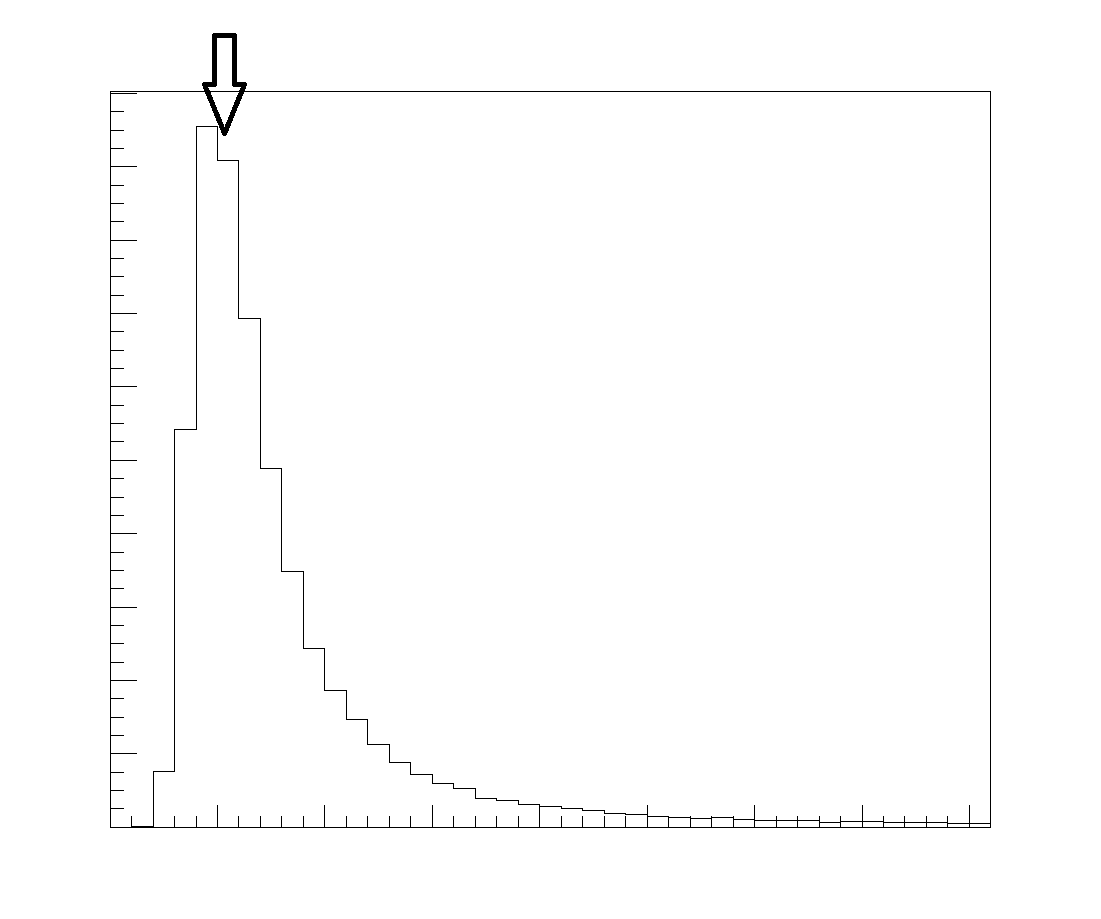
\includegraphics[width=0.5\columnwidth]{bilder/meanskizze}%
\caption{Schema der $E_T$-Mean-Analyse.}%
\label{fig:mean_skizze}%
\end{figure}

\begin{figure}%
\centering
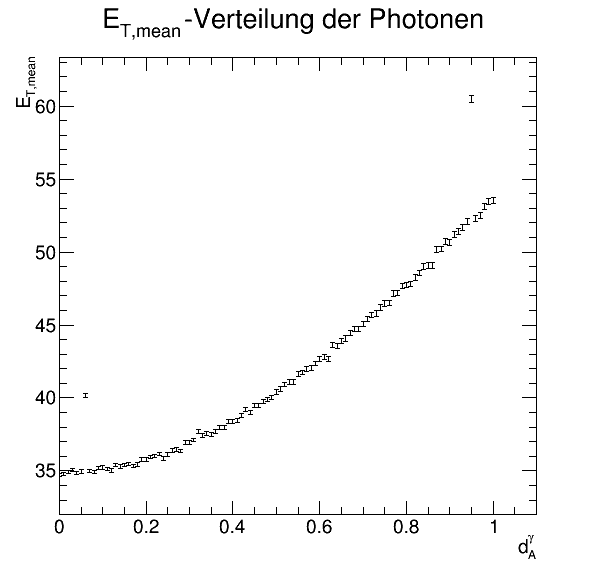
\includegraphics[width=0.5\columnwidth]{bilder/meanplot}%
\caption{Verlauf des Schwerpunktes der $E_T$-Verteilung.}%
\label{fig:mean_plot}%
\end{figure}

\subsection{Analyse der Einh�llenden der \texorpdfstring{$E_T$}{ET}-Verteilung}

\begin{figure}%
\centering
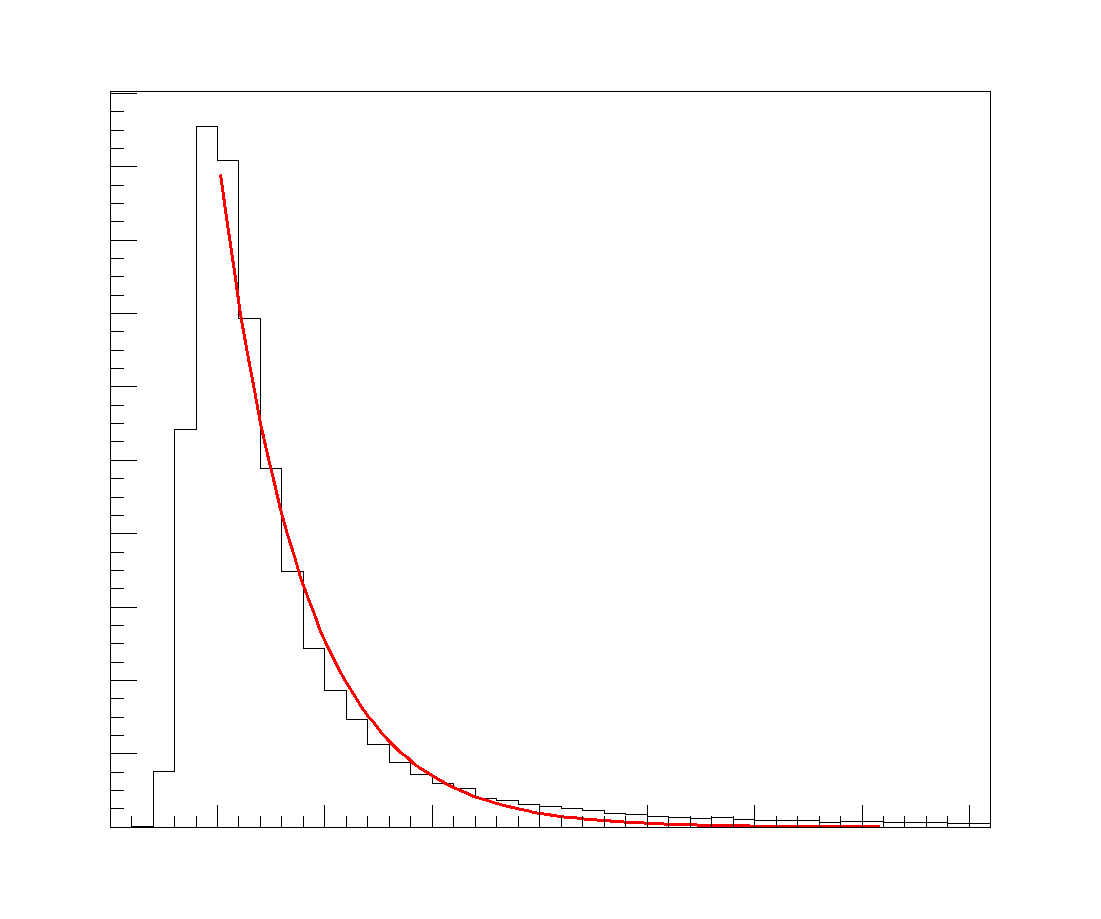
\includegraphics[width=0.5\columnwidth]{bilder/slopeskizze}%
\caption{Skizze zum Prinzip der Analyse der Einh�llenden.}%
\label{fig:slope_skizze}%
\end{figure}

Hier wird schlie�lich die Einh�llende der $E_T$-Verteilung betrachtet. Wie in Abb. \ref{fig:slope_skizze} zu sehen ist, kann die Verteilung im Bereich zwischen 50\,GeV und 200\,GeV durch eine logarithmische Funktion

\begin{equation}
N(x) = N_0\cdot e^{\lambda \cdot x}
\end{equation}

beschrieben werden. F�r jeden $d_A^{\gamma}$-Wert wird nun an das $E_T$-Spektrum eine Exponentialfunktion angefittet und der Wert von $\lambda$ gegen $d_A^{\gamma}$ aufgetragen. Dieser Plot ist in Abb. \ref{fig:slope_plot} zu sehen.

\begin{figure}%
\centering
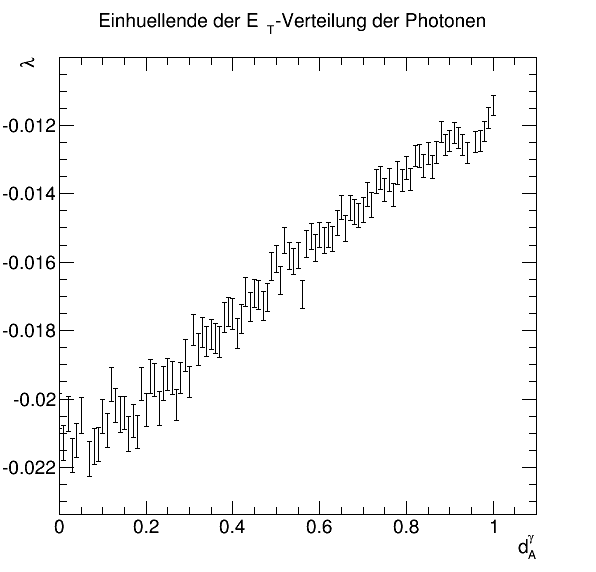
\includegraphics[width=0.5\columnwidth]{bilder/slopeplot}%
\caption{Verlauf der Einh�llenden der $E_T$-Verteilung.}%
\label{fig:slope_plot}%
\end{figure}
